\chapter{Wireshark results}

\begin{figure}[h!]
\begin{center}
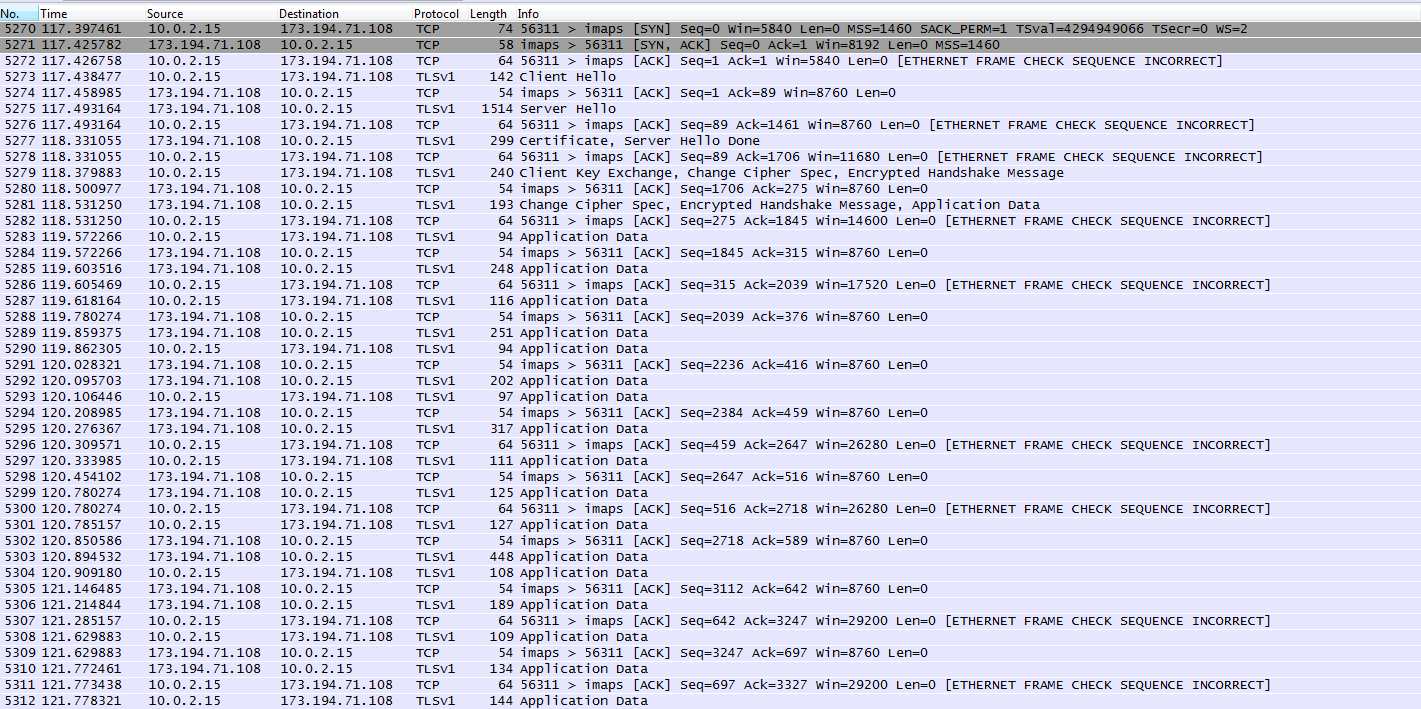
\includegraphics[height=0.6\textwidth, angle=-90]{ws1}
\end{center}
\caption{Traffic going to our application when recieving a single message} \label{fig:ws1}
\end{figure}

\begin{figure}[h!]
\begin{center}
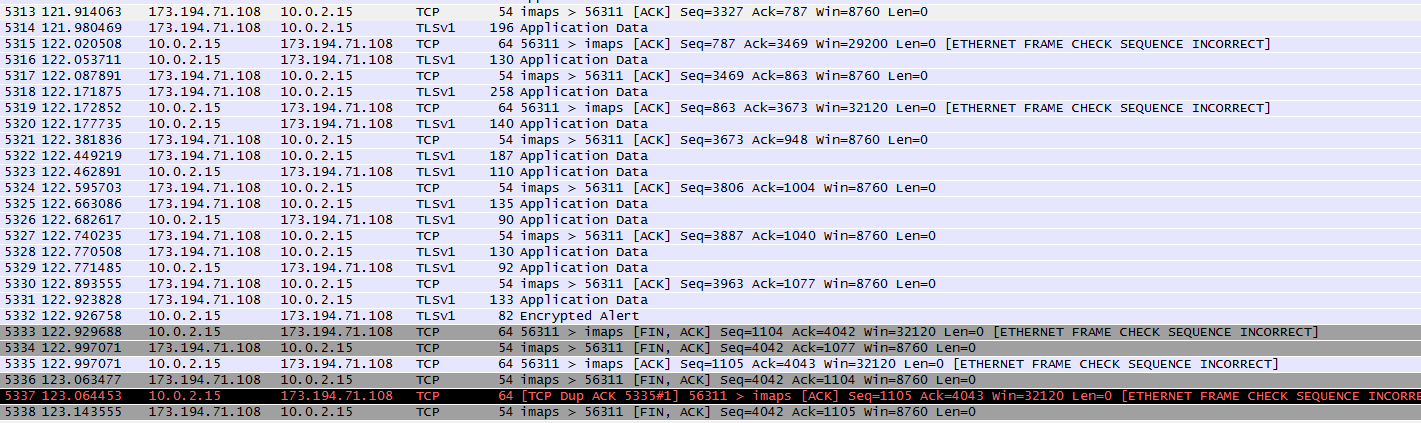
\includegraphics[height=0.38\textwidth, angle=-90]{ws2}
\end{center}
\caption{Traffic going from our application when recieving a single message} \label{fig:ws2}
\end{figure}

\begin{figure}[h!]
\begin{center}
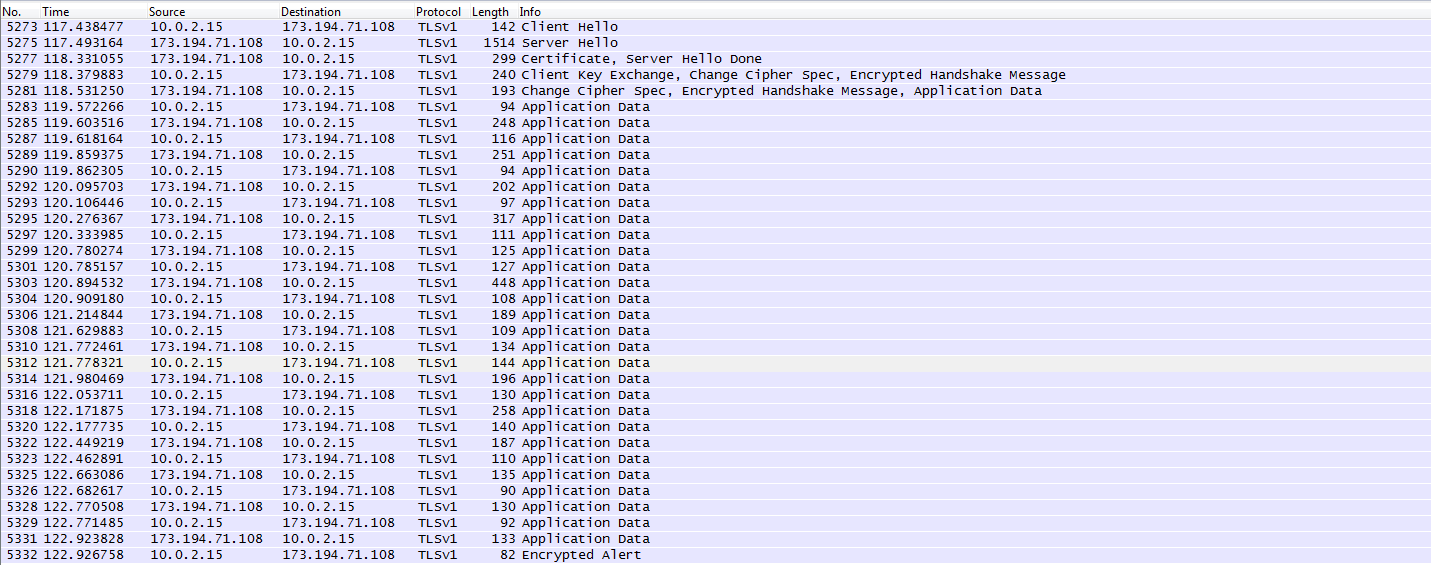
\includegraphics[height=0.5\textwidth, angle=-90]{ws3}
\end{center}
\caption{TLS packets sent to and from our application} \label{fig:ws3}
\end{figure}

\begin{figure}[h!]
\begin{center}
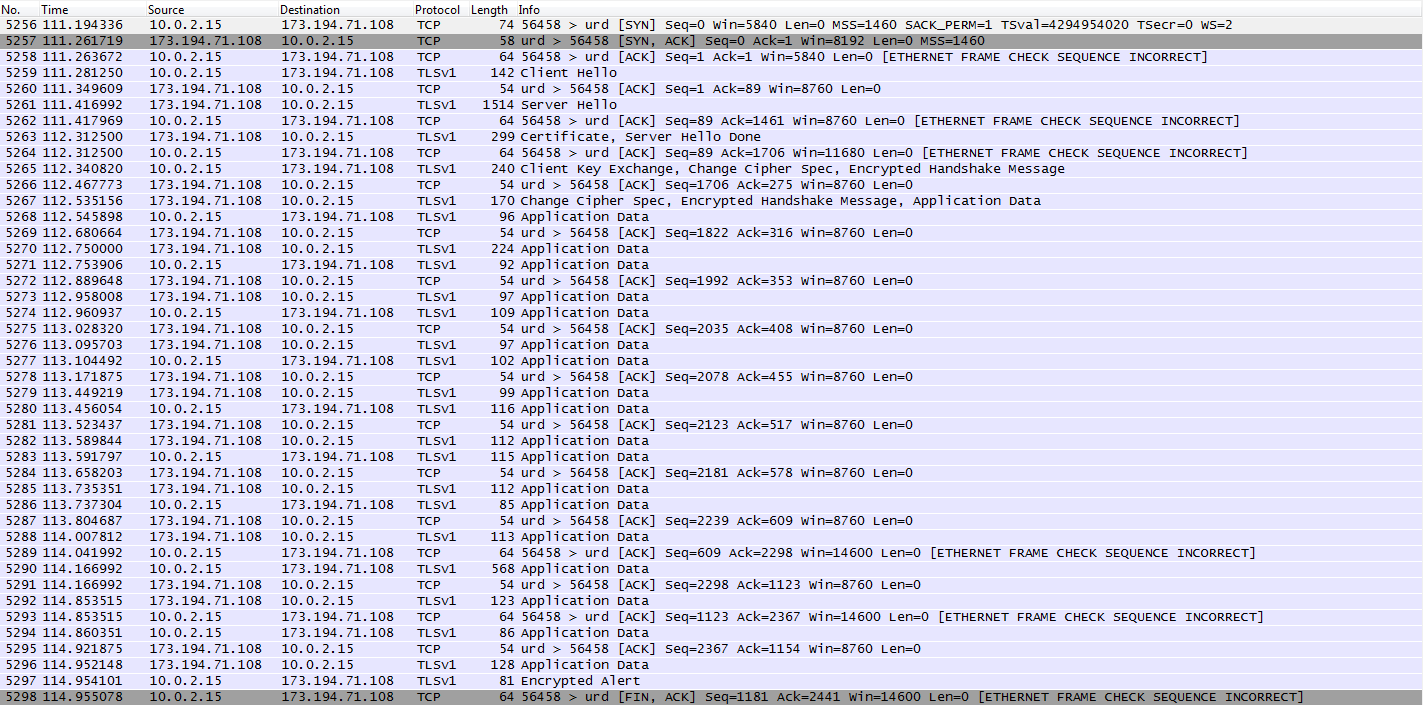
\includegraphics[height=0.6\textwidth, angle=-90]{ws4}
\end{center}
\caption{Traffic going to and from our application when sending a single message from our application} \label{fig:ws4}
\end{figure}

\begin{figure}[h!]
\begin{center}
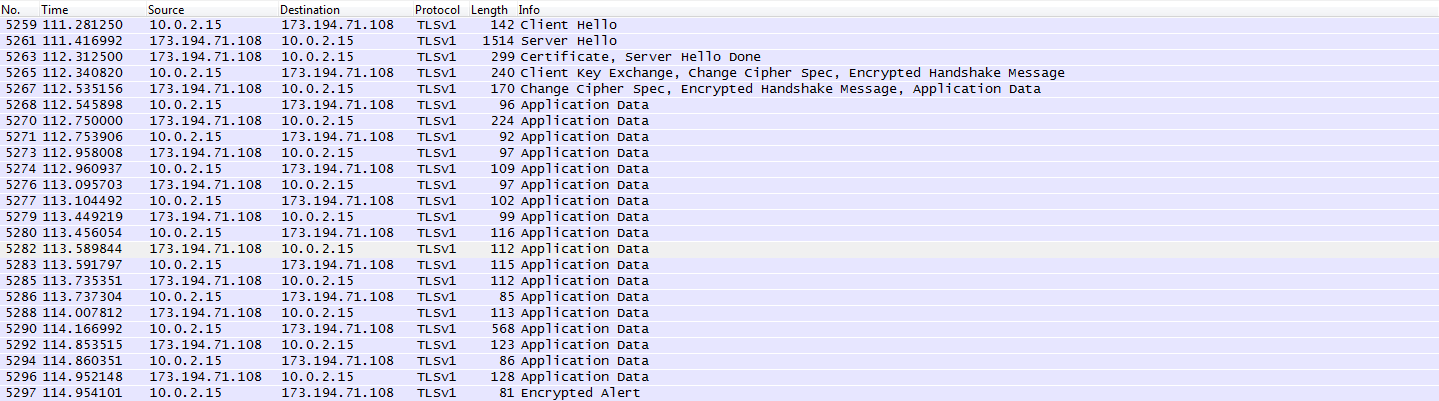
\includegraphics[height=0.35\textwidth, angle=-90]{ws5}
\end{center}
\caption{TLS packets sent to and from our application} \label{fig:ws5}
\end{figure}